% Asal-usul (tidak pernah dicetak): lihat sources/outline_sources.md (Tahun 1: kimia kristal
% mineral, silikat, larutan padat, rumus mineral, mineral pembentuk batuan utama). Kurva olivin
% di figdata/bachelor-1/solid_solution.py; analisis olivin pada soal rekaan (Fo sekitar 82);
% nilai soal dan masalah dalam skrip kalkulator scratch Buku 3 calc/ch07.py.
\chapter{Mineral pembentuk batuan}\label{ch:b1:rock-forming-minerals}

Meja dapur granit memperlihatkan tiga atau empat jenis butir: kuarsa abu-abu yang mengilap seperti kaca, \omterm{def:b1:rock-forming-minerals:groups}{feldspar} merah muda atau putih, serpihan \omterm{def:b1:rock-forming-minerals:groups}{mika} hitam. Pasir pantai hampir seluruhnya kuarsa. Kristal hijau kecil yang tersebar dalam basal adalah \omterm{def:b1:rock-forming-minerals:groups}{olivin}, dan \omterm{def:b1:rock-forming-minerals:mineral}{mineral} yang sama, dengan komposisi yang sedikit berbeda, membentuk sebagian besar mantel atas. Sejumlah kecil \omterm{def:b1:rock-forming-minerals:mineral}{mineral} membangun hampir setiap batuan, dan hampir semuanya silikat: oksigen dan silikon, dua unsur paling melimpah pada kerak, bergabung menjadi tetrahedron yang saling terhubung dengan beberapa cara sederhana. Bab ini menjelaskan bagaimana keterhubungan itu menentukan rumus dan habitus suatu silikat, bagaimana satu unsur menggantikan unsur lain dalam kristal sehingga suatu \omterm{def:b1:rock-forming-minerals:mineral}{mineral} berupa rentang komposisi, bukan satu komposisi saja, bagaimana analisis kimia menjadi rumus, dan apa saja \omterm{def:b1:rock-forming-minerals:mineral}{mineral} pembentuk batuan utama. Bab ini ditutup dengan \omterm{def:b1:rock-forming-minerals:groups}{olivin} dari basal yang dianalisis, dihitung ulang, dan ditimbang.

\begin{recall}
Kristal adalah padatan yang atom-atomnya berulang pada kisi; sel satuan adalah kotak terkecil yang berulang, dan bilangan koordinasi suatu ion menghitung tetangga terdekatnya yang bermuatan berlawanan (kimia, Sarjana Tahun ke-1). Jari-jari ion bergantung pada muatan dan pada koordinasinya. Suatu \omterm{def:b1:rock-forming-minerals:mineral}{mineral} dikenali di tangan dari habitusnya, belahannya, kekerasannya, dan kilapnya (Buku 2, kelas 11). Jumlah zat dihitung dalam mol, dan massa molar adalah massa satu mol (kimia).
\end{recall}

\section{Apa itu mineral}

\begin{definition}[Mineral]\label{def:b1:rock-forming-minerals:mineral}
Sebuah \emph{mineral}\index{mineral} adalah padatan yang terjadi secara alami dengan struktur kristal yang tertentu dan komposisi kimia yang tetap atau bervariasi dalam batas-batas tertentu. Hampir semua mineral bersifat anorganik.
\end{definition}

Sebuah batuan, sebaliknya, adalah agregat butir dari satu atau beberapa \omterm{def:b1:rock-forming-minerals:mineral}{mineral} (atau gelas): granit terdiri atas kuarsa, \omterm{def:b1:rock-forming-minerals:groups}{feldspar}, dan \omterm{def:b1:rock-forming-minerals:groups}{mika}; batu gamping sebagian besar kalsit. Kedua bagian definisi itu bersifat independen. Kaca jendela memiliki komposisi silikat tetapi tidak memiliki struktur kristal: ia bukan \omterm{def:b1:rock-forming-minerals:mineral}{mineral}, demikian pula gelas lava yang didinginkan dengan cepat. Sebaliknya, komposisi yang sama dapat mengkristal dalam beberapa struktur, dan setiap struktur adalah \omterm{def:b1:rock-forming-minerals:mineral}{mineral} yang berbeda.

\begin{definition}[Polimorf]\label{def:b1:rock-forming-minerals:polymorph}
Dua \omterm{def:b1:rock-forming-minerals:mineral}{mineral} adalah \emph{polimorf}\index{polimorf} satu sama lain bila keduanya memiliki komposisi kimia yang sama dan struktur kristal yang berbeda.
\end{definition}

Karbon mengkristal sebagai grafit, tumpukan lembaran heksagon dengan massa jenis \qty{2.16}{g.cm^{-3}}, dan sebagai intan, kerangka tempat setiap atom memiliki empat tetangga, dengan massa jenis \qty{3.51}{g.cm^{-3}}. Kalsium karbonat adalah kalsit (\qty{2.71}{g.cm^{-3}}) atau aragonit (\qty{2.93}{g.cm^{-3}}); silika adalah kuarsa (\qty{2.65}{g.cm^{-3}}) atau koesit (\qty{2.93}{g.cm^{-3}}); \ce{Al2SiO5} adalah kyanit (\qty{3.61}{g.cm^{-3}}), andalusit (\qty{3.15}{g.cm^{-3}}) atau silimanit (\qty{3.24}{g.cm^{-3}}).
% ledger: webmineral:polymorphs, hom:calcite, hom:quartz
Dalam setiap pasangan, \omterm{def:b1:rock-forming-minerals:polymorph}{polimorf} yang lebih padat adalah yang terbentuk pada tekanan yang lebih tinggi: pada suhu tertentu, menaikkan tekanan menguntungkan keadaan dengan volume yang lebih kecil (kimia, pergeseran kesetimbangan). Intan dalam kimberlit dan koesit dalam batuan yang dihantam meteorit karena itu mencatat tekanan yang hanya ditemukan jauh di dalam mantel atau dalam tumbukan. Tiga \omterm{def:b1:rock-forming-minerals:polymorph}{polimorf} \ce{Al2SiO5}, yang medan kestabilannya membagi bidang tekanan--suhu di antara mereka, digunakan untuk membaca kondisi metamorfisme (Sarjana Tahun ke-2).

\section{Tetrahedron silikat dan keterhubungannya}

Dalam setiap silikat umum, setiap atom silikon berada di pusat empat atom oksigen yang diletakkan di sudut-sudut tetrahedron beraturan: unit \ce{SiO4} yang telah dikenal dari kimia. Ion silikon kecil (\qty{0.26}{\angstrom} dalam koordinasi empat) dan ion oksida besar, sehingga empat oksigen muat mengelilinginya dan tidak lebih; ikatan silikon--oksigen kuat dan sebagian kovalen. Unit terisolasi membawa muatan $4 - 4\times2 = -4$.
% ledger: shannon:radii
Tetrahedron dapat berdiri sendiri, dengan muatannya diseimbangkan oleh kation logam di antaranya, atau berbagi sudut: oksigen yang dimiliki bersama oleh dua tetrahedron adalah oksigen \emph{penjembatan}. Dua tetrahedron tidak pernah berbagi rusuk atau bidang, yang akan membawa dua silikon terlalu dekat. Silikat diklasifikasikan menurut jumlah sudut yang dibagi setiap tetrahedron (\cref{def:b1:rock-forming-minerals:silicate-classes}).

\begin{omfigure}
\tikzset{
  tup/.pic={\filldraw[fill=omLithLime, draw=black, line join=round] (0,0) -- (1,0) -- (0.5,0.866) -- cycle;
            \fill[omThm] (0.5,0.2887) circle (0.11);},
  tdn/.pic={\filldraw[fill=omLithLime, draw=black, line join=round] (0,0) -- (1,0) -- (0.5,-0.866) -- cycle;
            \fill[omThm] (0.5,-0.2887) circle (0.11);},
  linkpanel/.style={x=0.45cm, y=0.45cm, baseline=(current bounding box.south)}}
\setlength{\tabcolsep}{4pt}
\begin{tabular}{cccc}
% (a) tetrahedron dalam perspektif
\begin{tikzpicture}[linkpanel]
  \useasboundingbox (-1.2,-1.0) rectangle (6.0,4.4);
  \coordinate (T) at (2.2,3.7); \coordinate (L) at (0.3,0.5); \coordinate (R) at (4.1,0.1);
  \coordinate (B) at (3.3,2.1); \coordinate (C) at (2.475,1.6);
  \draw[densely dashed, gray] (L) -- (B) -- (R) (B) -- (T);
  \shade[ball color=omLithShale] (B) circle (0.42);
  \draw[gray] (C) -- (T) (C) -- (L) (C) -- (R) (C) -- (B);
  \shade[ball color=omThm!70] (C) circle (0.24);
  \draw[thick, line join=round] (T) -- (L) -- (R) -- cycle;
  \foreach \p in {T,L,R} \shade[ball color=omLithShale] (\p) circle (0.42);
  \node[right] at (4.5,0.1) {\scriptsize O};
  \node[right] at (2.6,3.8) {\scriptsize O};
  \draw[omThm] (C) -- (4.6,2.2) node[right] {\scriptsize Si};
\end{tikzpicture} &
% (b) nesosilikat: tetrahedron terisolasi
\begin{tikzpicture}[linkpanel]
  \useasboundingbox (-1.2,-1.0) rectangle (6.0,4.4);
  \pic at (0,0.3) {tup}; \pic at (2.4,0.3) {tup}; \pic at (4.0,1.9) {tdn};
  \pic at (1.2,2.4) {tdn}; \pic at (3.0,2.8) {tup};
\end{tikzpicture} &
% (c) sorosilikat: pasangan
\begin{tikzpicture}[linkpanel]
  \useasboundingbox (-1.2,-1.0) rectangle (6.0,4.4);
  \pic at (0,0.9) {tup}; \pic at (1,0.9) {tdn};
  \pic at (2.6,2.6) {tup}; \pic at (3.6,2.6) {tdn};
\end{tikzpicture} &
% (d) siklosilikat: cincin enam
\begin{tikzpicture}[linkpanel]
  \useasboundingbox (-1.2,-1.0) rectangle (6.0,4.4);
  \begin{scope}[shift={(2.4,1.7)}]
  \foreach \t in {0,60,...,300} {
    \filldraw[fill=omLithLime, draw=black, line join=round] (\t-30:1) -- (\t+30:1) -- (\t:1.732) -- cycle;
    \fill[omThm] (\t:1.155) circle (0.11);}
  \end{scope}
\end{tikzpicture} \\
{\small (a) tetrahedron \ce{SiO4}} & {\small (b) \omterm{def:b1:rock-forming-minerals:silicate-classes}{nesosilikat}} & {\small (c) \omterm{def:b1:rock-forming-minerals:silicate-classes}{sorosilikat}} & {\small (d) \omterm{def:b1:rock-forming-minerals:silicate-classes}{siklosilikat}} \\
 & {\scriptsize $s = 0$, \ce{SiO4}} & {\scriptsize $s = 1$, \ce{Si2O7}} & {\scriptsize $s = 2$, \ce{Si6O18}} \\[6pt]
% (e) rantai tunggal
\begin{tikzpicture}[linkpanel]
  \useasboundingbox (-0.6,-1.2) rectangle (7.6,4.6);
  \begin{scope}[shift={(0,1.5)}]
  \foreach \i in {0,...,3} \pic at (2*\i,0) {tup};
  \foreach \i in {0,...,2} \pic at (2*\i+1,0) {tdn};
  \end{scope}
\end{tikzpicture} &
% (f) rantai ganda: dua rantai tunggal disambung melalui setiap puncak kedua
\begin{tikzpicture}[linkpanel]
  \useasboundingbox (-0.6,-1.2) rectangle (7.6,4.6);
  \begin{scope}[shift={(0.5,0.4)}]
  \foreach \i in {0,...,3} {\pic at (2*\i,0) {tup}; \pic at (2*\i,1.732) {tdn};}
  \foreach \i in {0,...,2} {\pic at (2*\i+1,0) {tdn}; \pic at (2*\i+1,1.732) {tup};}
  \end{scope}
\end{tikzpicture} &
% (g) lembaran
\begin{tikzpicture}[linkpanel]
  \useasboundingbox (-0.6,-1.2) rectangle (7.6,4.6);
  \foreach \j in {0,1,2} {
    \foreach \i in {0,1,2} {\pic at (2*\i+\j,1.732*\j) {tup};}
    \foreach \i in {0,1} {\pic at (2*\i+\j+1,1.732*\j) {tdn};}}
\end{tikzpicture} &
% (h) kerangka: lembaran yang puncaknya bergantian menghadap ke atas dan ke bawah
\begin{tikzpicture}[linkpanel]
  \useasboundingbox (-0.6,-1.2) rectangle (7.6,4.6);
  \foreach \j in {0,1,2} {
    \foreach \i in {0,1,2} {\pic at (2*\i+\j,1.732*\j) {tup};}
    \foreach \i in {0,1} {\pic at (2*\i+\j+1,1.732*\j) {tdn};}}
  \foreach \j in {0,1,2} \foreach \i in {0,1} {
    \filldraw[fill=white, draw=omThm, thick] (2*\i+\j+1.5,1.732*\j-0.2887) circle (0.17);}
\end{tikzpicture} \\
{\small (e) rantai tunggal} & {\small (f) rantai ganda} & {\small (g) lembaran} & {\small (h) kerangka} \\
{\scriptsize $s = 2$, \ce{SiO3}} & {\scriptsize $s = 2$ dan $3$, \ce{Si4O11}} & {\scriptsize $s = 3$, \ce{Si2O5}} & {\scriptsize $s = 4$, \ce{SiO2}} \\
\end{tabular}
\medskip

{\small Tetrahedron \ce{SiO4} (a) dan cara tetrahedron saling terhubung, dilihat dari atas: setiap segitiga adalah alas sebuah tetrahedron, dengan tiga oksigen di sudutnya, dan yang keempat di atas titik, yang menandai silikon. Sudut-sudut yang bersentuhan adalah oksigen yang dimiliki bersama; $s$ adalah jumlah sudut yang dibagi setiap tetrahedron. Dalam kerangka (h), oksigen puncak (lingkaran terbuka: menunjuk ke bawah; titik: menunjuk ke atas) juga dibagi, dengan lembaran di bawah dan di atasnya.}
\end{omfigure}

\begin{definition}[Kelas silikat]\label{def:b1:rock-forming-minerals:silicate-classes}
Silikat diklasifikasikan menurut cara tetrahedron \ce{SiO4}-nya terhubung. Dalam \emph{nesosilikat}\index{nesosilikat} tetrahedronnya terisolasi; dalam \emph{sorosilikat}\index{sorosilikat} mereka terhubung berpasangan oleh satu oksigen yang dimiliki bersama; dalam \emph{siklosilikat}\index{siklosilikat} mereka membentuk cincin tertutup, masing-masing berbagi dua sudut; dalam \emph{inosilikat}\index{inosilikat} mereka membentuk rantai tak berujung, tunggal (setiap tetrahedron berbagi dua sudut) atau ganda (dua rantai tunggal disambung berdampingan, separuh tetrahedron berbagi tiga sudut); dalam \emph{filosilikat}\index{filosilikat} mereka membentuk lembaran tak berujung, masing-masing berbagi tiga sudut; dalam \emph{tektosilikat}\index{tektosilikat} mereka membentuk kerangka tiga dimensi, masing-masing berbagi keempat sudutnya.
\end{definition}

\begin{proposition}[Rasio silikon terhadap oksigen]\label{prop:b1:rock-forming-minerals:si-o}
Jika setiap tetrahedron \ce{SiO4} suatu silikat rata-rata berbagi $s$ dari keempat sudutnya dengan tetrahedron lain, dan setiap oksigen yang dibagi tepat dimiliki oleh dua tetrahedron, maka jaringan silikat itu mengandung $4 - s/2$ oksigen per silikon, dan membawa muatan $s - 4$ per silikon.
\end{proposition}

\begin{proof}
Hitunglah oksigen tetrahedron demi tetrahedron. Sebuah tetrahedron dengan $s_i$ sudut yang dibagi memiliki $4 - s_i$ oksigen yang tidak dibagi sepenuhnya dan separuh dari masing-masing dari $s_i$ yang dibagi, karena setiap oksigen dihitung lagi oleh tetrahedron tetangga: ia menyumbang $4 - s_i + s_i/2 = 4 - s_i/2$ oksigen. Menjumlahkan atas $N$ tetrahedron dan membaginya dengan $N$ menghasilkan $4 - s/2$ oksigen per silikon, dengan $s$ rata-rata dari $s_i$. Setiap silikon membawa muatan $+4$ dan setiap oksigen $-2$, sehingga muatan per silikon adalah $4 - 2(4 - s/2) = s - 4$.
\end{proof}

Proposisi ini langsung memberikan anion setiap kelas. Tetrahedron terisolasi ($s = 0$): \ce{SiO4^{4-}}. Pasangan ($s = 1$): $4 - 1/2 = 7/2$, yaitu
\ce{Si2O7^{6-}}. Cincin dan rantai tunggal ($s = 2$): \ce{SiO3^{2-}}, ditulis
\ce{Si6O18^{12-}} untuk cincin enam, \ce{Si2O6^{4-}} untuk dua tetrahedron dari
rantai. Rantai ganda (separuh dengan $s = 2$, separuh dengan $s = 3$, sehingga $s = 5/2$):
$4 - 5/4 = 11/4$, \ce{Si4O11^{6-}}. Lembaran ($s = 3$): \ce{Si2O5^{2-}}.
Kerangka ($s = 4$): \ce{SiO2}, netral --- kuarsa adalah kerangka silikon dan oksigen saja. Makin banyak tetrahedron berbagi, makin kecil muatan yang perlu diseimbangkan dan makin sedikit kation logam: \omterm{def:b1:rock-forming-minerals:groups}{olivin} \ce{Mg2SiO4} memiliki dua ion logam per silikon, \omterm{def:b1:rock-forming-minerals:groups}{piroksen} seperti enstatit \ce{Mg2Si2O6} satu, kuarsa tidak ada.

Keterhubungan juga membentuk kristalnya. Silikat lembaran terbelah dengan mudah di antara lembarannya, tempat ikatannya lemah: \omterm{def:b1:rock-forming-minerals:groups}{mika} terkelupas menjadi serpih tipis yang lentur. Silikat rantai terbelah sejajar rantainya, sepanjang dua bidang dengan sudut yang ditentukan oleh cara rantai itu tersusun: sekitar \ang{87} dan \ang{93} pada \omterm{def:b1:rock-forming-minerals:groups}{piroksen}, yang rantainya sempit, dan \ang{56} dan \ang{124} pada \omterm{def:b1:rock-forming-minerals:groups}{amfibol}, yang rantai gandanya lebih lebar. Kedua sudut belahan itu, yang terlihat pada kristal yang pecah atau pada \omterm{def:b1:field-lab-methods-1:thin-section}{sayatan tipis}, adalah cara klasik untuk membedakan kedua kelompok.
% ledger: hom:diopside, hom:mg-hornblende

\section{Substitusi ionik dan larutan padat}

Kristal adalah himpunan situs, dan sebuah situs ditentukan oleh ukuran dan muatan yang dibutuhkannya, bukan oleh satu unsur. Sebuah ion dengan ukuran dan muatan yang tepat dapat menempati tempat ion lain dalam kristal yang sedang tumbuh, dan tidak ada batuan yang cukup murni untuk hanya menyediakan satu unsur.

\begin{definition}[Substitusi ionik, substitusi tergandeng]\label{def:b1:rock-forming-minerals:substitution}
Sebuah \emph{substitusi ionik}\index{substitusi ionik} adalah penggantian, dalam suatu situs struktur kristal, satu ion oleh ion lain dengan jari-jari yang serupa, tanpa perubahan struktur. Sebuah \emph{substitusi tergandeng}\index{substitusi tergandeng} adalah sepasang substitusi pada dua situs yang berbeda yang perubahan muatannya saling menghapus, sehingga kristal tetap netral.
\end{definition}

Dua aturan empiris, dari Goldschmidt, menyatakan substitusi mana yang mungkin. Jari-jarinya harus dekat: substitusi bebas bila keduanya berbeda kurang dari sekitar \qty{15}{\percent}, terbatas antara sekitar 15 dan \qty{30}{\percent}, dan jarang di atas itu. Muatannya tidak boleh berbeda lebih dari satu satuan, dan perbedaan muatan harus dikompensasi di tempat lain dalam struktur. Dalam situs enam-koordinasi \omterm{def:b1:rock-forming-minerals:groups}{olivin}, \ce{Mg^{2+}} (\qty{0.72}{\angstrom}) digantikan secara bebas oleh \ce{Fe^{2+}} (\qty{0.78}{\angstrom}, \qty{8}{\percent} lebih besar) dan oleh \ce{Ni^{2+}} (\qty{0.69}{\angstrom}), sedikit oleh \ce{Mn^{2+}} (\qty{0.83}{\angstrom}), hampir tidak oleh \ce{Ca^{2+}} (\qty{1.00}{\angstrom}, \qty{39}{\percent} lebih besar).
% ledger: goldschmidt:size, shannon:radii
Aturan-aturan ini adalah panduan: suhu memperlebar rentang yang mungkin, karena kristal panas menoleransi lebih banyak regangan, itulah sebabnya \omterm{def:b1:rock-forming-minerals:mineral}{mineral} yang tumbuh pada suhu tinggi sering mengandung lebih banyak ion yang tidak pas daripada \omterm{def:b1:rock-forming-minerals:mineral}{mineral} yang sama yang tumbuh dingin.

\begin{definition}[Larutan padat, anggota ujung]\label{def:b1:rock-forming-minerals:solid-solution}
Sebuah \emph{larutan padat}\index{larutan padat (mineral)} adalah \omterm{def:b1:rock-forming-minerals:mineral}{mineral} tempat satu atau lebih situs struktur ditempati, dalam proporsi yang bervariasi secara kontinu, oleh dua atau lebih ion. \emph{Anggota ujung}\index{anggota ujung} suatu larutan padat adalah komposisi pada batasnya, masing-masing dengan setiap situs yang bervariasi diisi oleh hanya satu ion; komposisi antara diberikan oleh fraksi mol anggota-anggota ujungnya.
\end{definition}

\omterm{def:b1:rock-forming-minerals:groups}{Olivin} adalah \omterm{def:b1:rock-forming-minerals:solid-solution}{larutan padat} antara forsterit \ce{Mg2SiO4} (Fo) dan fayalit \ce{Fe2SiO4} (Fa), lengkap dari satu \omterm{def:b1:rock-forming-minerals:solid-solution}{anggota ujung} ke yang lain: \omterm{def:b1:rock-forming-minerals:groups}{olivin} dengan \qty{82}{\percent} situs enam-koordinasinya diisi magnesium dan \qty{18}{\percent} oleh besi ditulis $\text{Fo}_{82}$, atau \ce{(Mg_{0.82}Fe_{0.18})2SiO4}. \omterm{def:b1:rock-forming-minerals:groups}{Garnet}, \omterm{def:b1:rock-forming-minerals:groups}{piroksen}, \omterm{def:b1:rock-forming-minerals:groups}{amfibol}, dan \omterm{def:b1:rock-forming-minerals:groups}{mika} adalah \omterm{def:b1:rock-forming-minerals:solid-solution}{larutan padat} dengan cara yang sama.
\omterm{def:b1:rock-forming-minerals:solid-solution}{larutan padat} dengan cara yang sama. \omterm{def:b1:rock-forming-minerals:groups}{Feldspar} \omterm{def:b1:rock-forming-minerals:groups}{plagioklas} adalah \omterm{def:b1:rock-forming-minerals:solid-solution}{larutan padat} dengan jenis yang berbeda, antara albit \ce{NaAlSi3O8} (Ab) dan anortit \ce{CaAl2Si2O8} (An). Natrium dan kalsium memiliki jari-jari yang hampir sama (\qty{1.02}{\angstrom} dan \qty{1.00}{\angstrom} dalam koordinasi enam) tetapi muatan yang berbeda; setiap kalsium yang masuk harus disertai aluminium yang menggantikan silikon dalam tetrahedron:
% ledger: shannon:radii
\[
  \mathrm{Na^{+}} + \mathrm{Si^{4+}} \;\rightleftharpoons\; \mathrm{Ca^{2+}} + \mathrm{Al^{3+}},
\]
\omterm{def:b1:rock-forming-minerals:substitution}{substitusi tergandeng} yang membiarkan muatan total tidak berubah.
Aluminium dapat masuk ke tetrahedron karena cukup kecil (\qty{0.39}{\angstrom} dalam koordinasi empat); ia adalah penggantian paling umum bagi silikon dalam silikat.

\begin{omfigure}
\begin{tikzpicture}[x=1cm, y=1cm,
  site/.style={draw, minimum width=1.25cm, minimum height=0.75cm, font=\small},
  asite/.style={site, fill=omLithGranite!60},
  tsite/.style={site, fill=omLithLime}]
\node[font=\small\bfseries, anchor=east] at (-0.4,1.6) {albit};
\node[asite] (a0) at (0.5,1.6) {$\mathrm{Na^{+}}$};
\node[tsite] (a1) at (2.2,1.6) {$\mathrm{Al^{3+}}$};
\node[tsite] (a2) at (3.55,1.6) {$\mathrm{Si^{4+}}$};
\node[tsite] (a3) at (4.9,1.6) {$\mathrm{Si^{4+}}$};
\node[tsite] (a4) at (6.25,1.6) {$\mathrm{Si^{4+}}$};
\node[anchor=west, font=\small] at (7.2,1.6) {$1 + 3 + 3\times4 = +16$, dengan \ce{O8}: $-16$};
\node[font=\small\bfseries, anchor=east] at (-0.4,-0.6) {anortit};
\node[asite] (b0) at (0.5,-0.6) {$\mathrm{Ca^{2+}}$};
\node[tsite] (b1) at (2.2,-0.6) {$\mathrm{Al^{3+}}$};
\node[tsite] (b2) at (3.55,-0.6) {$\mathrm{Al^{3+}}$};
\node[tsite] (b3) at (4.9,-0.6) {$\mathrm{Si^{4+}}$};
\node[tsite] (b4) at (6.25,-0.6) {$\mathrm{Si^{4+}}$};
\node[anchor=west, font=\small] at (7.2,-0.6) {$2 + 2\times3 + 2\times4 = +16$, dengan \ce{O8}: $-16$};
\draw[-{Stealth}, omThm, thick] (a0) -- node[left, font=\scriptsize] {$+1$} (b0);
\draw[-{Stealth}, omThm, thick] (a2) -- node[right, font=\scriptsize] {$-1$} (b2);
\node[font=\scriptsize] at (0.5,2.35) {situs besar};
\node[font=\scriptsize] at (4.22,2.35) {empat situs tetrahedral};
\end{tikzpicture}

{\small \omterm{def:b1:rock-forming-minerals:substitution}{Substitusi tergandeng} dalam \omterm{def:b1:rock-forming-minerals:groups}{plagioklas}. Penggantian natrium oleh kalsium pada situs besar menambah satu muatan positif; penggantian silikon oleh aluminium dalam tetrahedron menghapus satu. Setiap \omterm{def:b1:rock-forming-minerals:groups}{plagioklas} antara
$\mathrm{Na}_{1-x}\mathrm{Ca}_x\mathrm{Al}_{1+x}\mathrm{Si}_{3-x}\mathrm{O}_8$
adalah netral.}
\end{omfigure}

Sifat \omterm{def:b1:rock-forming-minerals:solid-solution}{larutan padat} bervariasi dengan komposisinya, dan inilah yang membuatnya berguna: massa jenis terukur, indeks bias, atau dimensi sel memberi komposisinya. Model paling sederhana memperlakukan \omterm{def:b1:rock-forming-minerals:solid-solution}{larutan padat} sebagai campuran ideal dalam volume: satu mol $\text{Fo}_x$ menempati volume $x$ mol forsterit dan $1 - x$ mol fayalit. Ini adalah model yang harus dibandingkan dengan pengukuran, dan ia sudah mengatakan sesuatu yang tidak jelas tentang massa jenisnya.

\begin{proposition}[Volume molar dan massa jenis larutan padat ideal]\label{prop:b1:rock-forming-minerals:ideal-mixing}
Misalkan dua \omterm{def:b1:rock-forming-minerals:solid-solution}{anggota ujung} memiliki massa molar $M_1$, $M_2$ dan volume molar
$V_1 = M_1/\rho_1$, $V_2 = M_2/\rho_2$. Dalam \omterm{def:b1:rock-forming-minerals:solid-solution}{larutan padat} dengan fraksi mol
$x$ \omterm{def:b1:rock-forming-minerals:solid-solution}{anggota ujung} 1, massa molarnya adalah
$M(x) = x M_1 + (1 - x) M_2$. Bila volume molarnya adalah
$V(x) = x V_1 + (1 - x) V_2$ (campuran ideal), massa jenisnya adalah
\[
  \rho(x) = \frac{x M_1 + (1 - x) M_2}{x V_1 + (1 - x) V_2},
\]
yang sama dengan $\rho_1$ pada $x = 1$ dan $\rho_2$ pada $x = 0$, dan merupakan fungsi linear dari $x$ hanya bila $V_1 = V_2$ atau $\rho_1 = \rho_2$.
\end{proposition}

\begin{proof}
Satu mol \omterm{def:b1:rock-forming-minerals:solid-solution}{larutan padat} mengandung $x$ mol unit rumus pertama dan $1 - x$ mol yang kedua; massanya $x M_1 + (1 - x) M_2$, volumenya $V(x)$ menurut hipotesis, dan $\rho = M/V$. Pada $x = 1$, $\rho = M_1/V_1 = \rho_1$; pada $x = 0$, $\rho = \rho_2$. Bila $V_1 = V_2$, $\rho = M(x)/V_1$ bersifat afin. Jika tidak, tulislah $\rho = (a + bx)/(c + dx)$ dengan $d = V_1 - V_2 \ne 0$. Bila ia afin, $p + qx$, maka $a + bx = (c + dx)(p + qx)$ untuk semua $x$, dan koefisien $x^2$ memberikan $qd = 0$, sehingga $q = 0$: $\rho$ akan konstan, $\rho_1 = \rho_2$. Sebaliknya, massa jenis \omterm{def:b1:rock-forming-minerals:solid-solution}{anggota ujung} yang sama membuat $\rho$ konstan.
\end{proof}

Untuk \omterm{def:b1:rock-forming-minerals:groups}{olivin}, dengan massa jenis terukur \qty{3.275}{g.cm^{-3}} untuk forsterit dan \qty{4.392}{g.cm^{-3}} untuk fayalit serta massa molar \qty{140.691}{g.mol^{-1}} dan \qty{203.771}{g.mol^{-1}}, volume molarnya adalah \qty{42.96}{cm^3.mol^{-1}} dan \qty{46.40}{cm^3.mol^{-1}}: mengganti magnesium dengan ion besi yang lebih besar memekarkan kristal sebesar \qty{8}{\percent}, dan menambah \qty{45}{\percent} pada massanya. Kurva massa jenis berada sedikit di atas garis lurus yang menghubungkan \omterm{def:b1:rock-forming-minerals:solid-solution}{anggota ujung}, hingga sekitar
\qty{0.02}{g.cm^{-3}} (\cref{exo:b1:rock-forming-minerals:10}): interpolasi garis lurus cukup dekat, tetapi tidak tepat.
% ledger: hom:forsterite, hom:fayalite, ciaaw:Mg, ciaaw:Fe, ciaaw:Si, ciaaw:O

\begin{omfigure}
\begin{tikzpicture}
\begin{axis}[name=vol, width=0.48\linewidth, height=5.2cm,
  xmin=0, xmax=100, ymin=42.5, ymax=46.8, xtick={0,20,...,100},
  tick label style={font=\scriptsize}, label style={font=\small},
  xlabel={kandungan forsterit (mol\,\%)}, ylabel={volume molar (\si{cm^3.mol^{-1}})},
  yticklabel style={/pgf/number format/fixed, /pgf/number format/precision=1}]
\addplot[omThm, thick] table[x=x_fo, y=V] {figdata/out/bachelor-1-solid_solution-curve.dat};
\node[font=\scriptsize, anchor=north west] at (axis cs:3,45.55) {fayalit};
\node[font=\scriptsize, anchor=north east] at (axis cs:97,42.95) {forsterit};
\end{axis}
\begin{axis}[at={(vol.east)}, anchor=west, xshift=1.3cm, width=0.48\linewidth, height=5.2cm,
  xmin=0, xmax=100, ymin=3.2, ymax=4.45, xtick={0,20,...,100},
  tick label style={font=\scriptsize}, label style={font=\small},
  xlabel={kandungan forsterit (mol\,\%)}, ylabel={massa jenis (\si{g.cm^{-3}})},
  yticklabel style={/pgf/number format/fixed, /pgf/number format/precision=1}]
\addplot[gray, densely dashed] table[x=x_fo, y=rho_lin] {figdata/out/bachelor-1-solid_solution-curve.dat};
\addplot[omThm, thick] table[x=x_fo, y=rho] {figdata/out/bachelor-1-solid_solution-curve.dat};
\end{axis}
\end{tikzpicture}

{\small \omterm{def:b1:rock-forming-minerals:solid-solution}{Larutan padat} \omterm{def:b1:rock-forming-minerals:groups}{olivin} sebagai campuran ideal forsterit dan fayalit, dari massa jenis terukurnya. Kiri: volume molar, linear dalam komposisi. Kanan: massa jenis (padat), sedikit di atas garis lurus di antara \omterm{def:b1:rock-forming-minerals:solid-solution}{anggota ujung} (putus-putus).}
\end{omfigure}

\section{Rumus mineral}

\begin{definition}[Rumus struktural, bilangan Mg]\label{def:b1:rock-forming-minerals:formula}
Sebuah \emph{rumus struktural}\index{rumus struktural (mineral)} suatu \omterm{def:b1:rock-forming-minerals:mineral}{mineral} memberikan, untuk jumlah atom oksigen yang tetap, jumlah atom setiap unsur dan situs yang ditempati masing-masing, dengan ion yang berbagi situs ditulis bersama: \omterm{def:b1:rock-forming-minerals:groups}{olivin}
$\mathrm{(Mg, Fe)_2SiO_4}$, sebuah \omterm{def:b1:rock-forming-minerals:groups}{plagioklas} $\mathrm{(Na_{0.5}Ca_{0.5})(Al_{1.5}Si_{2.5})O_8}$. \emph{Bilangan Mg}\index{bilangan Mg} suatu \omterm{def:b1:rock-forming-minerals:mineral}{mineral} atau batuan adalah
\[
  \mathrm{Mg\#} = 100\,\frac{\mathrm{Mg}}{\mathrm{Mg} + \mathrm{Fe^{2+}}},
\]
jumlah atom dihitung dalam mol (atau per unit rumus).
\end{definition}

Analisis kimia suatu \omterm{def:b1:rock-forming-minerals:mineral}{mineral}, dibuat dengan mikroprobe elektron pada \omterm{def:b1:field-lab-methods-1:thin-section}{sayatan tipis} yang dipoles (\cref{ch:b1:field-lab-methods-1}), tidak memberikan rumus: ia memberikan massa setiap unsur, yang menurut konvensi dilaporkan sebagai massa oksidanya, dalam persen massa sampel. Mengubah persentase ini menjadi rumus adalah perhitungan rutin.

\begin{method}[Menghitung ulang analisis pada jumlah oksigen tetap]\label{met:b1:rock-forming-minerals:recalculation}
Misalkan analisis memberikan oksida dalam persen berat, dan \omterm{def:b1:rock-forming-minerals:mineral}{mineralnya} memiliki
$n_O$ oksigen per unit rumus (4 untuk \omterm{def:b1:rock-forming-minerals:groups}{olivin}, 8 untuk \omterm{def:b1:rock-forming-minerals:groups}{feldspar}, 6 untuk
\omterm{def:b1:rock-forming-minerals:groups}{piroksen}, 12 untuk \omterm{def:b1:rock-forming-minerals:groups}{garnet}).
\begin{enumerate}
  \item Bagilah persen berat setiap oksida dengan massa molarnya: ini memberikan mol oksida dalam \qty{100}{g} \omterm{def:b1:rock-forming-minerals:mineral}{mineral}.
  \item Kalikan dengan jumlah oksigen dalam oksida (2 untuk \ce{SiO2}, 3 untuk \ce{Al2O3}, 1 untuk \ce{MgO}) untuk memperoleh mol oksigen, dan dengan jumlah kation dalam oksida (2 untuk \ce{Al2O3} dan \ce{Na2O}, 1 untuk \ce{SiO2}) untuk memperoleh mol kation.
  \item Jumlahkan mol oksigen, dan hitung faktornya,
        $f = n_O / \sum(\text{mol O})$.
  \item Kalikan setiap mol kation dengan $f$: hasilnya adalah atom setiap unsur per unit rumus.
  \item Tempatkan kation pada situs (silikon dan cukup aluminium untuk mengisi tetrahedron, sisanya pada situs yang lebih besar), dan periksa bahwa setiap situs memuat jumlah atom rumus ideal.
\end{enumerate}
\end{method}

Contoh terkerjakan: sebuah \omterm{def:b1:rock-forming-minerals:groups}{olivin} dengan \qty{40.80}{\percent} \ce{SiO2}, \qty{49.40}{\percent} \ce{MgO} dan \qty{9.80}{\percent} \ce{FeO}. Dengan massa molar \num{60.083}, \num{40.304} dan \qty{71.844}{g.mol^{-1}}, molnya dalam \qty{100}{g} adalah $0.67906$, $1.22568$ dan $0.13641$; oksigennya adalah $2\times0.67906 + 1.22568 + 0.13641 = 2.72021$, dan faktornya $f = 4/2.72021 = 1.47047$. Per empat oksigen: Si \num{0.999}, Mg \num{1.802}, Fe \num{0.201}. Situs tetrahedron memuat \num{0.999} atom dan situs oktahedral $1.802 + 0.201 = 2.003$, sangat dekat dengan 1 dan 2: analisisnya baik, dan \omterm{def:b1:rock-forming-minerals:groups}{olivinnya} adalah \ce{(Mg_{1.80}Fe_{0.20})SiO4}, $\text{Fo}_{90}$, dengan \omterm{def:b1:rock-forming-minerals:formula}{bilangan Mg} 90. Perhatikan bahwa muatannya menjumlah menjadi $2n_O = 8$ secara otomatis, apa pun analisisnya, selama setiap kation mempertahankan muatan oksidanya: perhitungan ulang itu sendiri membuat rumusnya netral. Jumlah situslah ujian yang sebenarnya.
% ledger: ciaaw:Si, ciaaw:Mg, ciaaw:Fe, ciaaw:O

Jumlah kation yang terlalu besar pada jumlah oksigen yang dipilih menyatakan bahwa sebagian besi adalah \ce{Fe^{3+}}, yang membawa lebih banyak oksigen per atom daripada yang diasumsikan analisis (\cref{exo:b1:rock-forming-minerals:12}); jumlah yang terlalu kecil, atau total jauh di bawah \qty{100}{\percent}, menyatakan bahwa ada sesuatu yang tidak dianalisis --- air dalam \omterm{def:b1:rock-forming-minerals:groups}{amfibol} atau \omterm{def:b1:rock-forming-minerals:groups}{mika}, karbon dioksida dalam karbonat. \omterm{def:b1:rock-forming-minerals:mineral}{Mineral} terhidrasi karena itu dihitung ulang pada oksigen tanpa airnya: 23 untuk \omterm{def:b1:rock-forming-minerals:groups}{amfibol} yang rumusnya memiliki \ce{O22(OH)2}, 22 untuk \omterm{def:b1:rock-forming-minerals:groups}{mika} dengan \ce{O20(OH)4} dalam unit rumus ganda.

\section{Mineral pembentuk batuan utama}

\begin{definition}[Kelompok mineral utama]\label{def:b1:rock-forming-minerals:groups}
\emph{Olivin}\index{olivin} adalah \omterm{def:b1:rock-forming-minerals:solid-solution}{larutan padat} \omterm{def:b1:rock-forming-minerals:silicate-classes}{nesosilikat} \ce{(Mg,Fe)2SiO4}. \emph{Garnet}\index{garnet} adalah kelompok \omterm{def:b1:rock-forming-minerals:silicate-classes}{nesosilikat} kubik $\mathrm{X_3Y_2(SiO_4)_3}$, X ion divalen (Mg, Fe, Mn, Ca), Y ion trivalen (Al, Fe, Cr). \emph{Piroksen}\index{piroksen} adalah \omterm{def:b1:rock-forming-minerals:silicate-classes}{inosilikat} rantai tunggal $\mathrm{XYSi_2O_6}$; \emph{amfibol}\index{amfibol} adalah \omterm{def:b1:rock-forming-minerals:silicate-classes}{inosilikat} rantai ganda dengan hidroksil, sekitar $\mathrm{A_{0-1}X_2Y_5(Si,Al)_8O_{22}(OH)_2}$. \emph{Mika}\index{mika} adalah silikat lembaran dengan ion kalium di antara lembarannya, seperti muskovit \ce{KAl2(Si3Al)O10(OH)2} dan biotit \ce{K(Mg,Fe)3(Si3Al)O10(OH)2}. \emph{Feldspar}\index{feldspar} adalah silikat kerangka aluminium dari natrium, kalium, atau kalsium. Feldspar \emph{plagioklas}\index{plagioklas} membentuk \omterm{def:b1:rock-forming-minerals:solid-solution}{larutan padat} albit \ce{NaAlSi3O8} -- anortit \ce{CaAl2Si2O8}; feldspar \emph{alkali}\index{feldspar alkali} terletak di antara albit dan ortoklas \ce{KAlSi3O8}.
\end{definition}

\begin{table}[htbp]
\centering\footnotesize
\setlength{\tabcolsep}{3pt}
% ledger: hom:forsterite, hom:fayalite, hom:almandine, webmineral:others, hom:diopside, hom:mg-hornblende, hom:muscovite, hom:biotite, hom:albite, hom:anorthite, hom:orthoclase, hom:quartz, hom:calcite, hom:magnetite
\begin{tabular}{@{}>{\raggedright\arraybackslash}p{1.6cm}>{\raggedright\arraybackslash}p{5.0cm}>{\raggedright\arraybackslash}p{1.7cm}>{\raggedright\arraybackslash}p{1.9cm}>{\raggedright\arraybackslash}p{1.3cm}>{\raggedright\arraybackslash}p{3.6cm}@{}}
\hline
kelompok & \omterm{def:b1:rock-forming-minerals:solid-solution}{anggota ujung}/contoh & kelas & massa jenis (\si{g.cm^{-3}}) & Mohs & belahan \\
\hline
\omterm{def:b1:rock-forming-minerals:groups}{olivin} & forsterit \ce{Mg2SiO4} -- fayalit \ce{Fe2SiO4} & neso & 3.28--4.39 & 6.5--7 & tidak sempurna; patahan konkoidal \\
\omterm{def:b1:rock-forming-minerals:groups}{garnet} & almandin \ce{Fe3Al2(SiO4)3}; pirop \ce{Mg3Al2(SiO4)3} & neso & 4.32; 3.74 & 7--7.5 & tidak ada \\
\omterm{def:b1:rock-forming-minerals:groups}{piroksen} & diopsid \ce{CaMgSi2O6}; enstatit \ce{Mg2Si2O6} & ino, rantai tunggal & 3.22--3.38; 3.2 & 5.5--6.5 & dua, pada sekitar \ang{87} dan \ang{93} \\
\omterm{def:b1:rock-forming-minerals:groups}{amfibol} & hornblende\newline \ce{Ca2(Mg,Fe)4Al(Si7Al)O22(OH)2} & ino, rantai ganda & 3.10--3.28 & 5--6 & dua, pada \ang{56} dan \ang{124} \\
\omterm{def:b1:rock-forming-minerals:groups}{mika} & muskovit \ce{KAl2(Si3Al)O10(OH)2};\newline biotit \ce{K(Mg,Fe)3(Si3Al)O10(OH)2} & filo & 2.77--2.88; 2.7--3.3 & 2.5--3 & satu, sempurna: serpih tipis \\
\omterm{def:b1:rock-forming-minerals:groups}{feldspar} & albit \ce{NaAlSi3O8}; anortit \ce{CaAl2Si2O8}; ortoklas \ce{KAlSi3O8} & tekto & 2.55--2.76 & 6--6.5 & dua baik, \{001\} dan \{010\} \\
kuarsa & \ce{SiO2} & tekto & 2.65 & 7 & tidak ada; patahan konkoidal \\
karbonat & kalsit \ce{CaCO3}; dolomit \ce{CaMg(CO3)2} & --- & 2.71; 2.84 & 3; 3.5--4 & tiga, rombohedral \\
oksida besi & magnetit \ce{Fe3O4} & --- & 5.18 & 5.5--6.5 & tidak ada; sangat magnetik \\
\hline
\end{tabular}
\caption{\omterm{def:b1:rock-forming-minerals:mineral}{Mineral} pembentuk batuan utama: rumus \omterm{def:b1:rock-forming-minerals:solid-solution}{anggota ujung} atau anggota umum, kelas struktural, massa jenis terukur dan kekerasan pada skala Mohs. Rentangnya adalah rentang \omterm{def:b1:rock-forming-minerals:solid-solution}{anggota ujung} atau sampel alami.}
\label{tab:b1:rock-forming-minerals:main}
\end{table}

\Cref{tab:b1:rock-forming-minerals:main} mengumpulkan \omterm{def:b1:rock-forming-minerals:mineral}{mineral-mineral} yang membentuk hampir semua batuan kerak dan mantel. Di mana mereka terjadi mengikuti dari kimianya dan dari kondisi tempat mereka mengkristal.

\emph{Silikat gelap.} \omterm{def:b1:rock-forming-minerals:groups}{Olivin}, \omterm{def:b1:rock-forming-minerals:groups}{piroksen}, \omterm{def:b1:rock-forming-minerals:groups}{amfibol}, biotit, dan banyak \omterm{def:b1:rock-forming-minerals:groups}{garnet} kaya magnesium dan besi; mereka padat dan gelap. \omterm{def:b1:rock-forming-minerals:groups}{Olivin} dan \omterm{def:b1:rock-forming-minerals:groups}{piroksen} mengkristal dari lelehan panas yang kaya magnesium: mereka adalah \omterm{def:b1:rock-forming-minerals:mineral}{mineral} basal dan gabro, serta peridotit mantel atas, yang sebagian besar berupa \omterm{def:b1:rock-forming-minerals:groups}{olivin}. \omterm{def:b1:rock-forming-minerals:groups}{Amfibol} dan biotit mengandung hidroksil dan memerlukan air dalam lelehan atau batuan: mereka terdapat dalam andesit, diorit, dan granit, dan dalam banyak batuan metamorf. \omterm{def:b1:rock-forming-minerals:groups}{Garnet} tumbuh terutama dalam batuan metamorf --- butir merah pada sekis \omterm{def:b1:rock-forming-minerals:groups}{mika} adalah almandin --- dan dalam batuan mantel dalam, tempat piropus stabil.

\emph{Silikat terang.} \omterm{def:b1:rock-forming-minerals:groups}{Feldspar}, kuarsa dan muskovit kaya silikon, aluminium, dan \omterm{def:b1:rock-forming-minerals:groups}{alkali}; mereka berwarna terang dan lebih ringan massa jenisnya. \omterm{def:b1:rock-forming-minerals:groups}{Feldspar} adalah \omterm{def:b1:rock-forming-minerals:mineral}{mineral} paling melimpah pada kerak: \omterm{def:b1:rock-forming-minerals:groups}{plagioklas} dalam basal, gabro, dan sebagian besar batuan beku lain, \omterm{def:b1:rock-forming-minerals:groups}{feldspar alkali} dalam granit. Kuarsa mengkristal paling akhir dari lelehan kaya silika, mengisi ruang di antara butir-butir lain dalam granit; karena ia keras, tanpa belahan, dan hampir tidak larut, ia bertahan dari pelapukan dan pengangkutan, dan menumpuk sebagai pasir. \omterm{def:b1:rock-forming-minerals:mineral}{Mineral} lempung, silikat lembaran yang terbentuk di permukaan, adalah pokok bahasan \cref{ch:b1:weathering-clays}.

\emph{Yang lain.} Kalsit dan dolomit membentuk batu gamping, batu dolomit, dan marmer; kalsit adalah satu-satunya \omterm{def:b1:rock-forming-minerals:mineral}{mineral} umum yang berdesis dalam asam encer dingin, dan ia pecah sepanjang tiga belahan menjadi rombohedron. Magnetit, hadir dalam jumlah kecil pada banyak batuan beku, membawa sebagian besar kemagnetannya, catatan yang dibaca oleh metode magnetik pada bab-bab berikutnya.


\subsection{Mineral dan massa jenis batuan}

Massa jenis suatu batuan mengikuti dari \omterm{def:b1:rock-forming-minerals:mineral}{mineralnya}. Jika batuan bebas pori tersusun dari \omterm{def:b1:rock-forming-minerals:mineral}{mineral} dengan fraksi volume $\varphi_i$ (berjumlah 1) dan massa jenis $\rho_i$, volume $V$ batuan mengandung massa
$\sum_i \varphi_i V \rho_i$, sehingga
\[
  \rho_{\text{batuan}} = \sum_i \varphi_i\,\rho_i ,
  \qquad
  w_i = \frac{\varphi_i\,\rho_i}{\rho_{\text{batuan}}},
\]
di mana $w_i$ adalah fraksi massa \omterm{def:b1:rock-forming-minerals:mineral}{mineral} $i$. Ambil granit dengan \qty{30}{\percent} kuarsa (\qty{2.65}{g.cm^{-3}}), \qty{60}{\percent} \omterm{def:b1:rock-forming-minerals:groups}{feldspar} (sekitar \qty{2.62}{g.cm^{-3}}) dan \qty{10}{\percent} biotit (sekitar \qty{3.0}{g.cm^{-3}}), dan gabro dengan \qty{55}{\percent} \omterm{def:b1:rock-forming-minerals:groups}{plagioklas} (sekitar \qty{2.72}{g.cm^{-3}}), \qty{35}{\percent} \omterm{def:b1:rock-forming-minerals:groups}{piroksen} (sekitar \qty{3.30}{g.cm^{-3}}) dan \qty{10}{\percent} \omterm{def:b1:rock-forming-minerals:groups}{olivin} (sekitar \qty{3.45}{g.cm^{-3}}), masing-masing massa jenis dipilih dalam rentang \cref{tab:b1:rock-forming-minerals:main}. Maka
\begin{align*}
  \rho_{\text{granit}} &= 0.30\times2.65 + 0.60\times2.62 + 0.10\times3.0
  = \qty{2.67}{g.cm^{-3}},\\
  \rho_{\text{gabro}} &= 0.55\times2.72 + 0.35\times3.30 + 0.10\times3.45
  = \qty{3.00}{g.cm^{-3}}.
\end{align*}
Selisihnya, sekitar \qty{12}{\percent}, berasal dari silikat gelap: besi dan magnesium yang tidak dimiliki granit. Itulah sebabnya benua, yang sebagian besar tersusun dari batuan granitik, berdiri lebih tinggi daripada dasar samudra dari basal dan gabro, suatu keseimbangan yang dibahas dalam \cref{ch:b1:isostasy-gravity}. Dalam gabro, \omterm{def:b1:rock-forming-minerals:groups}{olivin} adalah \qty{10}{\percent} volumenya tetapi $0.10\times3.45/3.00 = \qty{11.5}{\percent}$ massanya: \omterm{def:b1:rock-forming-minerals:mineral}{mineral} padat lebih berat dalam batuan daripada bagiannya dalam volume.

\begin{inthelab}[Membedakan mineral]
% ledger: commons:min-calcite
\begin{minipage}[t]{0.58\linewidth}\vspace{0pt}
Di laboratorium, seorang mineralog yang mengidentifikasi spesimen tangan menguji sifat-sifat \cref{tab:b1:rock-forming-minerals:main} satu per satu: kekerasan terhadap ujung baja dan lempeng kaca, belahan pada permukaan patah yang segar, massa jenis dari berat spesimen di udara dan di air, dan, untuk karbonat, reaksi dengan setetes asam klorida encer dingin di bawah pengisapan asap. Belahan kalsit adalah kasus buku teks: sebuah kristal pecah berulang kali menjadi rombohedron yang lebih kecil dengan sudut yang sama. Butir yang terlalu kecil untuk dikenali dengan tangan diidentifikasi pada \omterm{def:b1:field-lab-methods-1:thin-section}{sayatan tipis} dengan \omterm{def:b1:field-lab-methods-1:microscope}{mikroskop polarisasi} (\cref{ch:b1:optical-mineralogy}), dan komposisi tepatnya dengan analisis mikroprobe, dihitung ulang seperti dalam \cref{met:b1:rock-forming-minerals:recalculation}.
\end{minipage}\hfill
\begin{minipage}[t]{0.39\linewidth}\vspace{0pt}
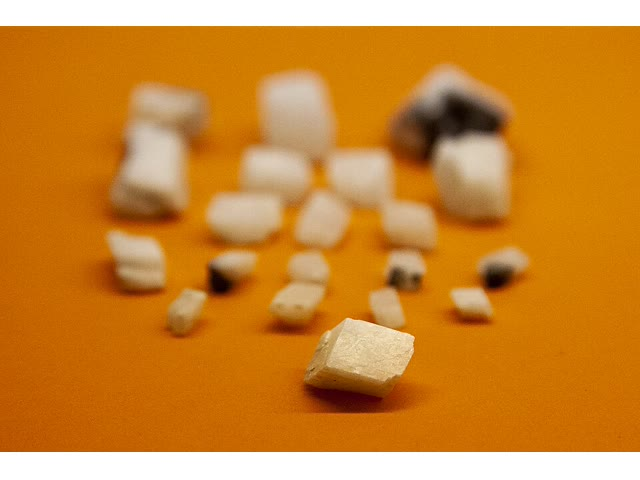
\includegraphics[width=\linewidth]{images/book3/b1-mineral-calcite-rhombs.jpg}

{\scriptsize Rombohedron belahan kalsit. Foto Giovanna Canu dan Eva Santini, CC BY 4.0 (Wikimedia Commons).}
\end{minipage}
\end{inthelab}

\begin{omfigure}
\setlength{\tabcolsep}{2pt}
\begin{tabular}{ccc}
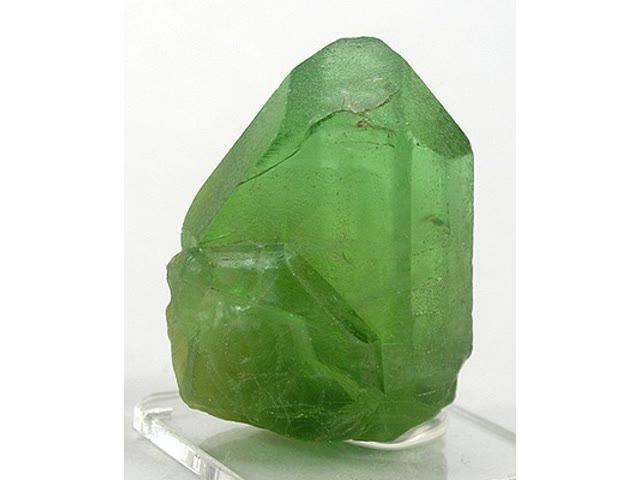
\includegraphics[width=0.31\linewidth]{images/book3/b1-mineral-olivine.jpg} &
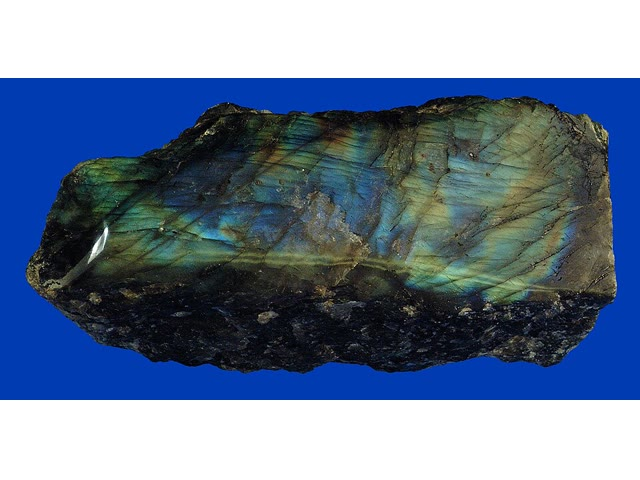
\includegraphics[width=0.31\linewidth]{images/book3/b1-mineral-plagioclase.jpg} &
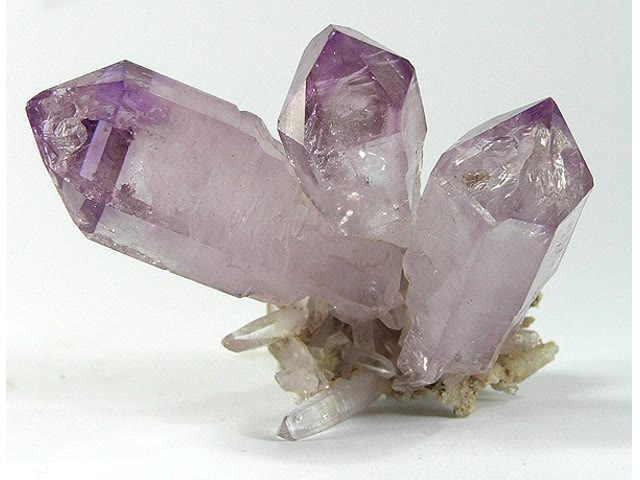
\includegraphics[width=0.31\linewidth]{images/book3/b1-mineral-quartz.jpg} \\
{\small (a) \omterm{def:b1:rock-forming-minerals:groups}{olivin}} & {\small (b) \omterm{def:b1:rock-forming-minerals:groups}{plagioklas} (labradorit)} & {\small (c) kuarsa (ametis)} \\[4pt]
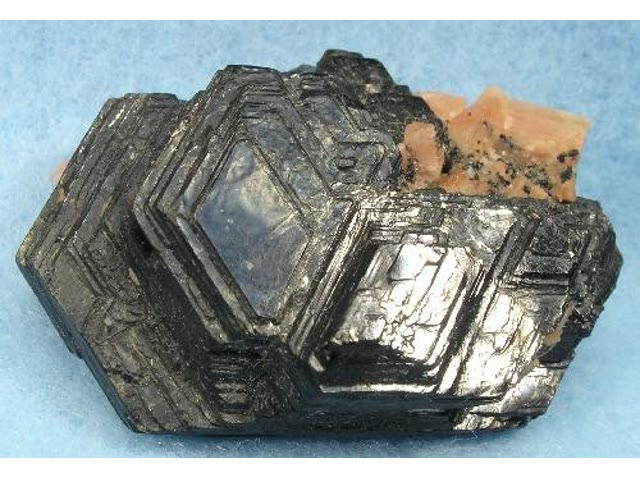
\includegraphics[width=0.31\linewidth]{images/book3/b1-mineral-biotite.jpg} &
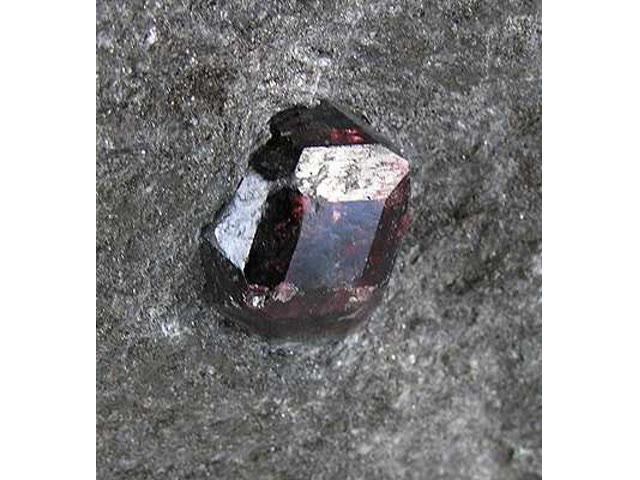
\includegraphics[width=0.31\linewidth]{images/book3/b1-mineral-garnet.jpg} &
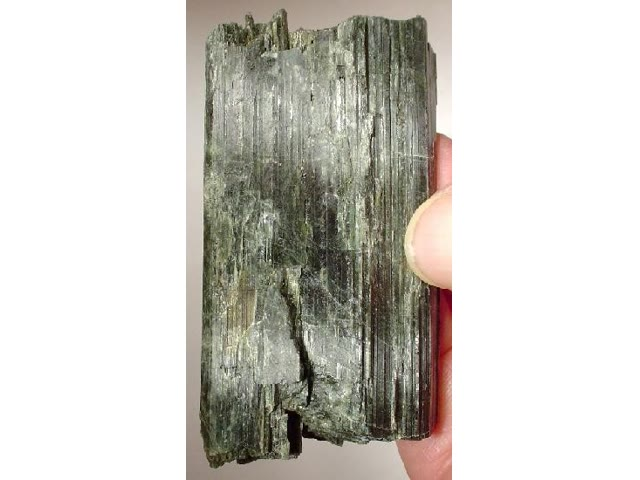
\includegraphics[width=0.31\linewidth]{images/book3/b1-mineral-hornblende.jpg} \\
{\small (d) biotit di atas ortoklas} & {\small (e) \omterm{def:b1:rock-forming-minerals:groups}{garnet} (almandin)} & {\small (f) hornblende} \\
\end{tabular}
\medskip
% ledger: commons:min-olivine, commons:min-plagioclase, commons:min-quartz, commons:min-biotite, commons:min-garnet, commons:min-hornblende

{\small Enam \omterm{def:b1:rock-forming-minerals:mineral}{mineral} pembentuk batuan: (a) kristal \omterm{def:b1:rock-forming-minerals:groups}{olivin} permata; (b) lempeng \omterm{def:b1:rock-forming-minerals:groups}{plagioklas} yang dipoles memperlihatkan permainan warna labradorit; (c) kristal kuarsa, prisma enam sisi dengan ujung piramidal; (d) tumpukan serpihan biotit di atas kristal ortoklas; (e) kristal \omterm{def:b1:rock-forming-minerals:groups}{garnet} almandin dalam matriksnya; (f) prisma hornblende. Foto (a), (c)--(f) Robert M.~Lavinsky, CC BY-SA 3.0; (b) Twyla Baker, CC0 (Wikimedia Commons).}
\end{omfigure}

\section{Latihan}

\begin{exercise}[$\star$]\label{exo:b1:rock-forming-minerals:1}
Sebutkan kelas silikat setiap anion, dan berikan jumlah $s$ sudut yang dibagi setiap tetrahedron: \ce{SiO4^{4-}}, \ce{Si2O7^{6-}}, \ce{Si6O18^{12-}}, \ce{Si2O5^{2-}}, \ce{SiO2}. Kelas manakah yang dapat dimiliki \ce{SiO3^{2-}}?
\end{exercise}

\begin{exercise}[$\star$]\label{exo:b1:rock-forming-minerals:2}
Dengan massa atom O \num{15.999}, Si \num{28.085}, Mg \num{24.305} dan Fe \qty{55.845}{g.mol^{-1}}, hitunglah massa molar forsterit dan fayalit, lalu volume molarnya dari massa jenis \num{3.275} dan \qty{4.392}{g.cm^{-3}}.
% ledger: ciaaw:O, ciaaw:Si, ciaaw:Mg, ciaaw:Fe, hom:forsterite, hom:fayalite
\end{exercise}

\begin{exercise}[$\star$]\label{exo:b1:rock-forming-minerals:3}
Dengan koordinasi enam, jari-jari ionnya adalah \ce{Mg^{2+}} \qty{0.72}{\angstrom}, \ce{Fe^{2+}} \qty{0.78}{\angstrom}, \ce{Ni^{2+}} \qty{0.69}{\angstrom}, \ce{Mn^{2+}} \qty{0.83}{\angstrom} dan \ce{Ca^{2+}} \qty{1.00}{\angstrom}. Hitunglah selisih setiap jari-jari itu dari jari-jari \ce{Mg^{2+}} dalam persen, dan nyatakan, menurut aturan Goldschmidt, ion mana yang dapat menggantikan magnesium secara bebas dalam \omterm{def:b1:rock-forming-minerals:groups}{olivin}.
% ledger: shannon:radii, goldschmidt:size
\end{exercise}

\begin{exercise}[$\star$]\label{exo:b1:rock-forming-minerals:4}
Grafit dan intan memiliki massa jenis \num{2.16} dan \qty{3.51}{g.cm^{-3}}; kalsit dan aragonit \num{2.71} dan \qty{2.93}{g.cm^{-3}}. Dengan berapa persen massa jenis naik pada setiap perubahan? \omterm{def:b1:rock-forming-minerals:polymorph}{Polimorf} manakah dari setiap pasangan yang terbentuk pada tekanan yang lebih tinggi?
% ledger: webmineral:polymorphs, hom:calcite
\end{exercise}

\begin{exercise}[$\star\star$]\label{exo:b1:rock-forming-minerals:5}
Tulislah \omterm{def:b1:rock-forming-minerals:formula}{rumus struktural} \omterm{def:b1:rock-forming-minerals:groups}{plagioklas} $\text{An}_{30}$ (\qty{30}{\percent}
dari situs besar terisi kalsium), dan periksalah bahwa ia netral.
\end{exercise}

\begin{exercise}[$\star\star$]\label{exo:b1:rock-forming-minerals:6}
Dalam rantai ganda, separuh tetrahedron berbagi dua sudut dan separuh berbagi tiga. Hitunglah oksigen suatu kelompok berulang dari empat tetrahedron langsung pada panel (f) dari figur keterhubungan, dan periksa rumus \ce{Si4O11^{6-}} yang diberikan oleh \cref{prop:b1:rock-forming-minerals:si-o}.
\end{exercise}

\begin{exercise}[$\star\star$]\label{exo:b1:rock-forming-minerals:7}
Hitunglah ulang analisis \omterm{def:b1:rock-forming-minerals:groups}{olivin} \qty{40.20}{\percent}
\ce{SiO2}, \qty{47.10}{\percent} \ce{MgO}, \qty{12.20}{\percent} \ce{FeO},
\qty{0.40}{\percent} \ce{NiO} (massa molar \ce{NiO}
\qty{74.692}{g.mol^{-1}}) pada empat oksigen.
Berikan \omterm{def:b1:rock-forming-minerals:formula}{rumus strukturalnya}, periksa, dan berikan kandungan forsteritnya.
Kemudian tunjukkan bahwa kandungan forsterit dapat dicari dari persentase \ce{MgO} dan \ce{FeO} saja.
\end{exercise}

\begin{exercise}[$\star\star$]\label{exo:b1:rock-forming-minerals:8}
Periksalah bahwa muskovit \ce{KAl2(Si3Al)O10(OH)2} netral. Lembaran tetrahedronnya memiliki satu aluminium untuk tiga silikon: muatan apa yang diberikan ini kepada lembaran per unit rumus, dan ion apa yang menyeimbangkannya?
\end{exercise}

\begin{exercise}[$\star\star$]\label{exo:b1:rock-forming-minerals:9}
Dengan memakai volume molar \num{42.96} dan \qty{46.40}{cm^3.mol^{-1}} dan massa molar \num{140.691} dan \qty{203.771}{g.mol^{-1}}: (a) hitunglah massa jenis $\text{Fo}_{50}$ dengan campuran ideal, dan bandingkan dengan rata-rata massa jenis \omterm{def:b1:rock-forming-minerals:solid-solution}{anggota ujungnya}; (b) carilah kandungan forsterit suatu \omterm{def:b1:rock-forming-minerals:groups}{olivin} dengan massa jenis \qty{3.600}{g.cm^{-3}}.
\end{exercise}

\begin{exercise}[$\star\star\star$]\label{exo:b1:rock-forming-minerals:10}
Dengan notasi \cref{prop:b1:rock-forming-minerals:ideal-mixing}, tunjukkan
bahwa
\[
  \rho(x) - \bigl(x\rho_1 + (1 - x)\rho_2\bigr) =
  \frac{x(1 - x)(\rho_1 - \rho_2)(V_1 - V_2)}{V(x)} .
\]
Simpulkan bahwa massa jenis \omterm{def:b1:rock-forming-minerals:groups}{olivin} berada di atas garis lurus di antara \omterm{def:b1:rock-forming-minerals:solid-solution}{anggota ujung}, dan hitunglah selisihnya pada $\text{Fo}_{50}$.
\end{exercise}

\begin{exercise}[$\star\star\star$]\label{exo:b1:rock-forming-minerals:11}
Sebuah \omterm{def:b1:rock-forming-minerals:groups}{plagioklas} dari gabro memberikan \qty{54.10}{\percent} \ce{SiO2},
\qty{28.90}{\percent} \ce{Al2O3}, \qty{11.20}{\percent} \ce{CaO},
\qty{5.10}{\percent} \ce{Na2O} dan \qty{0.30}{\percent} \ce{K2O} (massa molar
\num{60.083}, \num{101.961}, \num{56.077}, \num{61.979},
\qty{94.195}{g.mol^{-1}}). Hitunglah ulang pada delapan oksigen; periksa bahwa situs tetrahedron (Si + Al) memuat 4 atom dan situs besar (Ca + Na + K) 1; periksa \omterm{def:b1:rock-forming-minerals:substitution}{substitusi tergandeng} dengan membandingkan $\mathrm{Al} - 1$ dengan Ca; berikan kandungan anortit $100\,\mathrm{Ca}/(\mathrm{Ca} +
\mathrm{Na} + \mathrm{K})$.
\end{exercise}

\begin{exercise}[$\star\star\star$]\label{exo:b1:rock-forming-minerals:12}
Mikroprobe tidak dapat membedakan \ce{Fe^{2+}} dari \ce{Fe^{3+}} dan melaporkan semua besi sebagai \ce{FeO}. (a) Tunjukkan bahwa magnetit murni \ce{Fe3O4}, yang dianalisis dengan cara ini, berjumlah \qty{93.09}{\percent}. (b) Hitunglah ulang analisis ini pada empat oksigen, dan jelaskan mengapa hasilnya mustahil untuk \omterm{def:b1:rock-forming-minerals:mineral}{mineral} dengan tiga kation per empat oksigen. (c) Hitunglah ulang pada tiga kation sebagai gantinya, dan temukan jumlah \ce{Fe^{2+}} dan \ce{Fe^{3+}} dengan mensyaratkan rumus netral. (d) Nyatakan ulang analisis sebagai \ce{FeO} dan \ce{Fe2O3}, dan berikan totalnya yang baru.
\end{exercise}

\section{Soal: Olivin dari basal}

\begin{problem}[{Soal akhir pekan --- menghitung ulang analisis mikroprobe suatu olivin, menulis dan memeriksa rumusnya, serta mencari komposisi, massa jenis, dan massanya dalam satu meter kubik basal}]
\label{pb:b1:rock-forming-minerals:1}
% analisis rekaan: figdata/bachelor-1/solid_solution.py (OLIVINE_WT); nilai: calc/ch07.py
% ledger: ciaaw:O, ciaaw:Si, ciaaw:Mg, ciaaw:Fe, ciaaw:Mn, ciaaw:Ni, ciaaw:Ca, hom:forsterite, hom:fayalite, shannon:radii
Kristal hijau basal adalah \omterm{def:b1:rock-forming-minerals:groups}{olivin}. Analisis mikroprobe salah satu dari mereka memberikan, dalam persen berat oksida:
\begin{center}
\small
\begin{tabular}{lcccccc}
\hline
oksida & \ce{SiO2} & \ce{FeO} & \ce{MnO} & \ce{MgO} & \ce{NiO} & \ce{CaO} \\
berat \% & 39.50 & 16.53 & 0.23 & 43.32 & 0.20 & 0.22 \\
\hline
\end{tabular}
\end{center}
Massa atom adalah O \num{15.999}, Si \num{28.085}, Fe \num{55.845}, Mn
\num{54.938}, Mg \num{24.305}, Ni \num{58.693}, Ca \qty{40.078}{g.mol^{-1}}.
Forsterit memiliki massa jenis \qty{3.275}{g.cm^{-3}} dan fayalit
\qty{4.392}{g.cm^{-3}}.

\medskip
\noindent\textbf{Bagian I --- Dari oksida ke kation.}
\begin{enumerate}
  \item Hitunglah massa molar keenam oksida.
  \item Hitunglah total analisis. Apa yang disarankan oleh total \qty{97}{\percent}?
  \item Hitunglah jumlah mol setiap oksida dalam \qty{100}{g} \omterm{def:b1:rock-forming-minerals:groups}{olivin}.
  \item Hitunglah mol oksigen yang dikandungnya, dan jumlahnya.
  \item Hitunglah mol setiap kation.
  \item Hitunglah faktor yang membawa oksigen menjadi empat.
  \item Berikan jumlah atom setiap unsur per empat oksigen, hingga tiga desimal.
\end{enumerate}

\medskip
\noindent\textbf{Bagian II --- Rumus struktural.}
\begin{enumerate}[resume]
  \item \omterm{def:b1:rock-forming-minerals:groups}{Olivin} memiliki satu situs tetrahedral dan dua situs oktahedral per empat oksigen. Hitunglah jumlah kation selain silikon, dan bandingkan kedua total situs dengan rumus ideal.
  \item Tulislah \omterm{def:b1:rock-forming-minerals:formula}{rumus struktural} \omterm{def:b1:rock-forming-minerals:groups}{olivin}.
  \item Periksa bahwa rumusnya netral, dan jelaskan mengapa pemeriksaan ini, tidak seperti milik soal 8, tidak mungkin gagal.
  \item Dengan memakai jari-jari ion (\ce{Mg^{2+}} \qty{0.72}{\angstrom},
        \ce{Fe^{2+}} \qty{0.78}{\angstrom}, \ce{Ni^{2+}}
        \qty{0.69}{\angstrom}, \ce{Mn^{2+}} \qty{0.83}{\angstrom},
        \ce{Ca^{2+}} \qty{1.00}{\angstrom}, semuanya dalam koordinasi enam), jelaskan mengapa nikel umum dalam \omterm{def:b1:rock-forming-minerals:groups}{olivin} dan kalsium jarang.
  \item Mikroprobe melaporkan semua besi sebagai \ce{FeO}. Jelaskan mengapa jumlah kation yang ditemukan pada soal 7 menunjukkan bahwa \omterm{def:b1:rock-forming-minerals:groups}{olivin} tidak mengandung \ce{Fe^{3+}} yang berarti.
\end{enumerate}

\medskip
\noindent\textbf{Bagian III --- Komposisi.}
\begin{enumerate}[resume]
  \item Hitunglah kandungan forsterit $\mathrm{Fo} = 100\,\mathrm{Mg}/(\mathrm{Mg} +
        \mathrm{Fe})$, hingga satu desimal.
  \item Berapakah \omterm{def:b1:rock-forming-minerals:formula}{bilangan Mg} \omterm{def:b1:rock-forming-minerals:groups}{olivin}? Mengapa ia sama dengan kandungan forsterit di sini?
  \item Tulislah \omterm{def:b1:rock-forming-minerals:groups}{olivin} sebagai \omterm{def:b1:rock-forming-minerals:solid-solution}{larutan padat} biner
        $\mathrm{Fo}_x\mathrm{Fa}_{1-x}$, dengan mengabaikan Mn, Ni dan Ca, dan berikan proporsi situs oktahedralnya yang berisi besi.
  \item Tunjukkan bahwa kandungan forsterit dapat dihitung dari persentase \ce{MgO} dan \ce{FeO} saja, tanpa faktor soal 6, dan lakukanlah.
  \item Sebuah \omterm{def:b1:rock-forming-minerals:groups}{olivin} yang tumbuh kemudian dalam lava yang sama memiliki \qty{40.5}{\percent} \ce{MgO} dan \qty{20.0}{\percent} \ce{FeO}. Hitunglah kandungan forsteritnya. \omterm{def:b1:rock-forming-minerals:groups}{Olivin} mana yang lebih kaya besi?
\end{enumerate}

\medskip
\noindent\textbf{Bagian IV --- Massa jenis dan massa.}
\begin{enumerate}[resume]
  \item Hitunglah massa molar dan volume molar forsterit dan fayalit (volume molar hingga dua desimal).
  \item Dengan menganggap \omterm{def:b1:rock-forming-minerals:groups}{olivin} sebagai biner $\mathrm{Fo}_x\mathrm{Fa}_{1-x}$ dari soal 15, dengan $x$ dibulatkan hingga tiga desimal, hitunglah massa molar dan volume molarnya dengan campuran ideal.
  \item Turunkan massa jenisnya, hingga tiga desimal.
  \item Bandingkan dengan interpolasi garis lurus di antara massa jenis \omterm{def:b1:rock-forming-minerals:solid-solution}{anggota ujung}.
  \item Basal mengandung \qty{12}{\percent} \omterm{def:b1:rock-forming-minerals:groups}{olivin} menurut volume. Berapa massa \omterm{def:b1:rock-forming-minerals:groups}{olivin} yang dikandung satu meter kubik basal?
  \item Basal memiliki massa jenis \qty{2.95}{g.cm^{-3}}. Berapa proporsi \omterm{def:b1:rock-forming-minerals:groups}{olivin} menurut massa?
  \item Berapakah kandungan forsterit \omterm{def:b1:rock-forming-minerals:groups}{olivin}, dibulatkan ke persen utuh terdekat?
\end{enumerate}
\end{problem}
